\section{Algorithms}

\begin{frame}{Graph-based ANNS Algorithms}
    Two phases:
    \begin{enumerate}
        \item Index construction
        \item (Greedy) Search 
    \end{enumerate}
\end{frame}

\subsection{Search}

\begin{frame}{\textsc{GreedySearch}}
    \begin{figure}[h]
        \centering
        \hfill
        \begin{subfigure}{0.31\textwidth}
            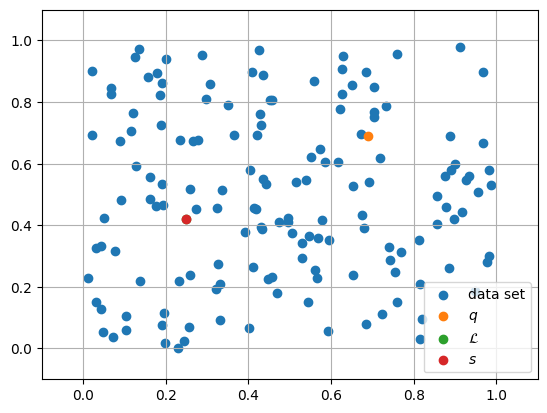
\includegraphics[width=\textwidth]{images/greedy-search-begin}
            \caption{Initialization}
        \end{subfigure}
        \hfill
        \begin{subfigure}{0.31\textwidth}
            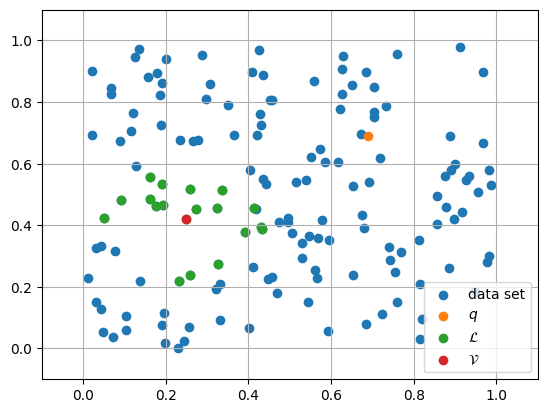
\includegraphics[width=\textwidth]{images/greedy-search-1}
            \caption{Iteration 1}
        \end{subfigure}
        \hfill
        \begin{subfigure}{0.31\textwidth}
            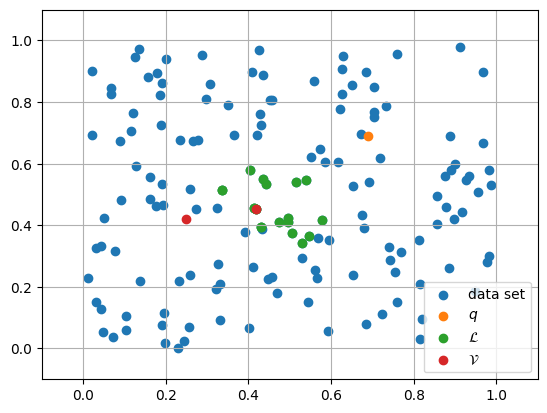
\includegraphics[width=\textwidth]{images/greedy-search-2}
            \caption{Iteration 2}
        \end{subfigure}
        \hfill
    \end{figure}
\end{frame}

\begin{frame}{\textsc{GreedySearch}}
    \begin{figure}[h]
        \centering
        \hfill
        \begin{subfigure}{0.31\textwidth}
            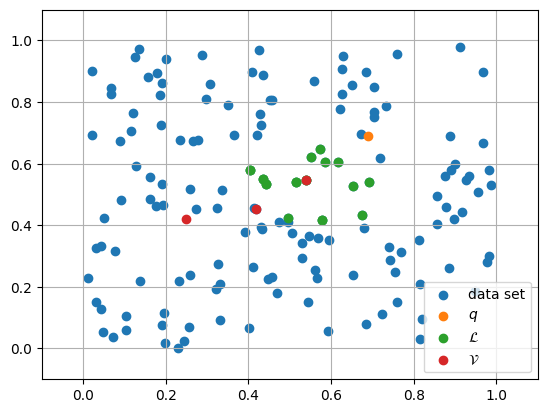
\includegraphics[width=\textwidth]{images/greedy-search-3}
            \caption{Iteration 3}
        \end{subfigure}
        \hfill
        \begin{subfigure}{0.31\textwidth}
            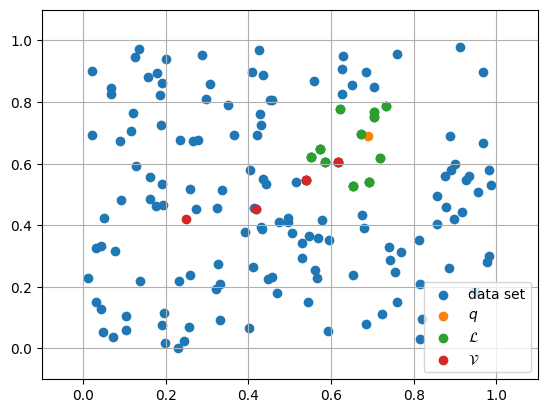
\includegraphics[width=\textwidth]{images/greedy-search-4}
            \caption{Iteration 4}
        \end{subfigure}
        \hfill
        \begin{subfigure}{0.31\textwidth}
            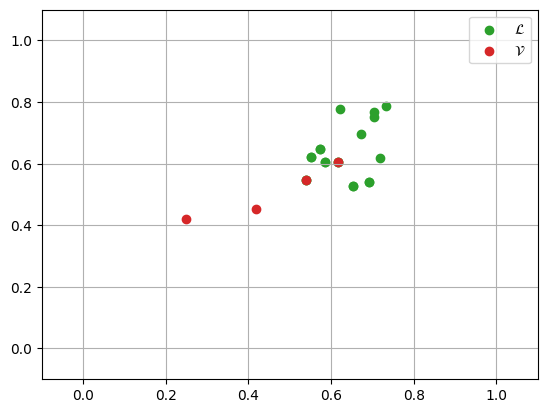
\includegraphics[width=\textwidth]{images/greedy-search-final}
            \caption{Returning values}
        \end{subfigure}
        \hfill
    \end{figure}
\end{frame}

\begin{frame}{\textsc{GreedySearch} Algorithm}
    \begin{algorithm}[H]
        \caption{\textsc{GreedySearch}(Query \(q\), Starting \(s\), Max queue size \(L\))}\label{alg:greedy-search}
        \begin{algorithmic}[1]
            % \Function{GreedySearch}{\(G, s, q, k, L\){}}
            %     \State{\(\mathcal{L} \gets \left\{s\right\}\); \(\mathcal{V} \gets \emptyset\)} \Comment{candidates \(\mathcal{L}\), visited \(\mathcal{V}\)}
            %     \While{\(\mathcal{L} \setminus \mathcal{V} \neq \emptyset\)}
            %         \State{\(p^* \gets \arg\min_{p \in \mathcal{L} \setminus \mathcal{V}} \delta(p, q)\)}
            %         \State{\(\mathcal{L} \gets \mathcal{L} \cup N_{\text{out}}(p^*)\)}
            %         \State{\(\mathcal{V} \gets \mathcal{V} \cup \left\{p^*\right\}\)}
            %         \If{\(|\mathcal{L}| > L\)}
            %             \State{\(\mathcal{L} \gets \textsc{GetClosest}(\mathcal{L}, L)\)}
            %         \EndIf
            %     \EndWhile
            %     \State{\Return{\(\mathcal{L}, \mathcal{V}\)}}
            % \EndFunction
            \State{Init \(\mathcal{L}\) as work queue with \(s\)}
            \State{Init \(\mathcal{V}\) to store visited vertices}
            \While{\(\mathcal{L}\) contains unvisited vertices}
                \State{Let \(p^*\) be point closest to \(q\) in \(\mathcal{L}\)}
                \State{Add \(N(p^*)\) to \(\mathcal{L}\)}
                \State{Mark \(p^*\) as visited}
                \If{\(|\mathcal{L}| > L\)}
                    \State{Pick \(L\) points closest to \(q\) in \(\mathcal{L}\) to keep}
                \EndIf
            \EndWhile
            \State{\Return{\([\mathcal{L}, \mathcal{V}]\)}}
        \end{algorithmic}
    \end{algorithm}
\end{frame}

\subsection{Index Construction}

\begin{frame}{Index Construction}
    In the ANNScaling paper, there are two outstanding performers:
    \begin{itemize}
        \item Hierarchical Navigable Small World
            \begin{itemize}
                \item Multi-layer proximity graph
                \item Shows up the most in ANNS-related literature
            \end{itemize}
        \item DiskANN
            \begin{itemize}
                \item Intuitively HNSW squashed down into 1 layer + directed
            \end{itemize}
    \end{itemize}
\end{frame}

\subsection{HNSW}

\begin{frame}
\begin{algorithm}[H]
    \caption{SelectNeighbors Algorithm}\label{alg:select-nbrs}
    \begin{algorithmic}[1]
        \Function{SelectNeighbors}{\(G, q, \mathcal{C}, M\){}}
            \State{\(\mathcal{R} \gets \emptyset\); \(\mathcal{W} \gets \mathcal{C}\)} \Comment{keepers \(\mathcal{R}\), candidates \(\mathcal{W}\)}
            \While{\(|\mathcal{W}| > 0\) and \(|\mathcal{R}| < M\)}
                \State{\(p^* \gets \arg\min_{p \in \mathcal{W}} \delta(p, q)\)}
                \If{\(\delta(p^*, q) < \min_{p' \in \mathcal{R}} \delta(p', q)\)}
                    \State{\(\mathcal{R} \gets \mathcal{R} \cup \left\{e\right\}\)}
                \EndIf
            \EndWhile
            \State{\Return{\(\mathcal{R}\)}}
        \EndFunction
    \end{algorithmic}
\end{algorithm}

\textbf{Inputs:} Graph \(G\), Query \(q\), Candidates \(\mathcal{C}\), Max degree \(M\)
\end{frame}

\begin{frame}
\begin{algorithm}[H]
    \caption{HNSW Algorithm}\label{alg:hnsw}
    \begin{algorithmic}[1]
        \Function{HNSW}{\(\mathcal{P}, C, M, m_L\)}
            \State{\(G \gets\) empty graph}
            \For{\(p \in \mathcal{P}\)}
                \State{\(\mathcal{W} \gets \emptyset\), \(ep \gets s\)}
            \EndFor
            \State{\Return{\(G\)}}
        \EndFunction
    \end{algorithmic}
\end{algorithm}

\textbf{Inputs:} Point set \(\mathcal{P}\)
\end{frame}

\subsection{DiskANN}

\begin{frame}
\begin{algorithm}[H]
    \caption{RobustPrune Algorithm}\label{alg:robust-prune}
    \begin{algorithmic}[1]
        \Procedure{RobustPrune}{\(G, p, \mathcal{V}, \alpha, M\){}}
            \State{\(\mathcal{V} \gets \mathcal{V} \cup N_{\text{out}}(p) \setminus \left\{p\right\};N_\text{out}(p) \gets \emptyset\)}
            \While{\(\mathcal{V} \neq \emptyset\)}
                \State{\(p^* \gets \arg\min_{p \in \mathcal{V}} \delta(p, q)\)}
                \State{\(N_\text{out}(p) \gets N_\text{out}(p) \cup \left\{p^*\right\}\)}
                \If{\(|N_\text{out}(p) = M\)}
                    \State{break}
                \EndIf
                \For{\(p' \in \mathcal{V}\)}
                    \If{\(\alpha \cdot \delta(p^*, p') \leq \delta(p, p')\)}
                        \State{\(\mathcal{V} \gets \mathcal{V} \setminus \left\{p'\right\}\)}
                    \EndIf
                \EndFor
            \EndWhile
        \EndProcedure
    \end{algorithmic}
\end{algorithm}

\textbf{Inputs:} Graph \(G\), Starting point \(p\), Candidate set \(\mathcal{V}\), Distance scaler \(\alpha\), Max degree \(M\)
\end{frame}

\begin{frame}
\begin{algorithm}[H]
    \caption{Vamana Algorithm}\label{alg:vamana}
    \begin{algorithmic}[1]
        \Function{Vamana}{\(\mathcal{P}, \alpha, C, M\){}}
            \State{Initialize \(G\) as random directed graph with max degree \(M\)}
            \State{\(s \gets \textsc{Medoid}(\mathcal{P})\); \(n \gets |\mathcal{P}|\)}
            \For{\(p \in \mathcal{P}\)}
                \State{\(\mathcal{L}, \mathcal{V} \gets \textsc{GreedySearch}(s, p, 1, C)\)}
                \State{\(\textsc{RobustPrune}(p, \mathcal{V}, \alpha, M)\)}
                \For{\(p' \in N_\text{out}(p)\)}
                    \If{\(|N_\text{out}(p') \cup \left\{p'\right\}| > M\)}
                        \State{\(\textsc{RobustPrune}(p', N_\text{out}(p')\cup\left\{p'\right\}, \alpha, M)\)}
                    \Else
                        \State{\(N_\text{out}(p') \gets N_\text{out}(p') \cup \left\{p'\right\}\)}
                    \EndIf
                \EndFor
            \EndFor
            \State{\Return{\(G\)}}
        \EndFunction
    \end{algorithmic}
\end{algorithm}

\textbf{Inputs:} Point set \(\mathcal{P}\), Dist. scaler \(\alpha\), Candidate size \(C\), Max degree \(M\)
\end{frame}
